\chapter{Dasar Teori}
\section{OpenStreetMap}
OpenStreetMap (OSM) adalah portal peta terbuka yang menyediakan data dalam bentuk peta atau 
XML \cite{wiki:001}. OSM menyediakan peta dijital dan dapat diedit dari seluruh
dunia, juga memungkinkan pengguna untuk mengakses gambar peta yang terdapat pada
situs \url{www.openstreetmap.org} secara gratis. OSM terbentuk dan mendapatkan
datanya dari berbagai sukarelawan yang bersedia untuk berkontribusi, misalnya para pengguna OSM yang menggunakan aplikasi untuk 
mengedit peta dan mengunggah data yang telah diedit ke situs OSM. Selain itu, OSM menyediakan 
beberapa aplikasi bagi para pengguna untuk mengedit peta, seperti iD online editor dan JOSM. 
Untuk mendapatkan gambar peta ataupun data peta dalam bentuk lain, pengguna dapat menggunakan 
fitur export pada situs OSM. Fitur export pada situs OSM dapat
dilihat pada Gambar \ref{fig:export_osm}.
\begin{figure}[h]
\centering
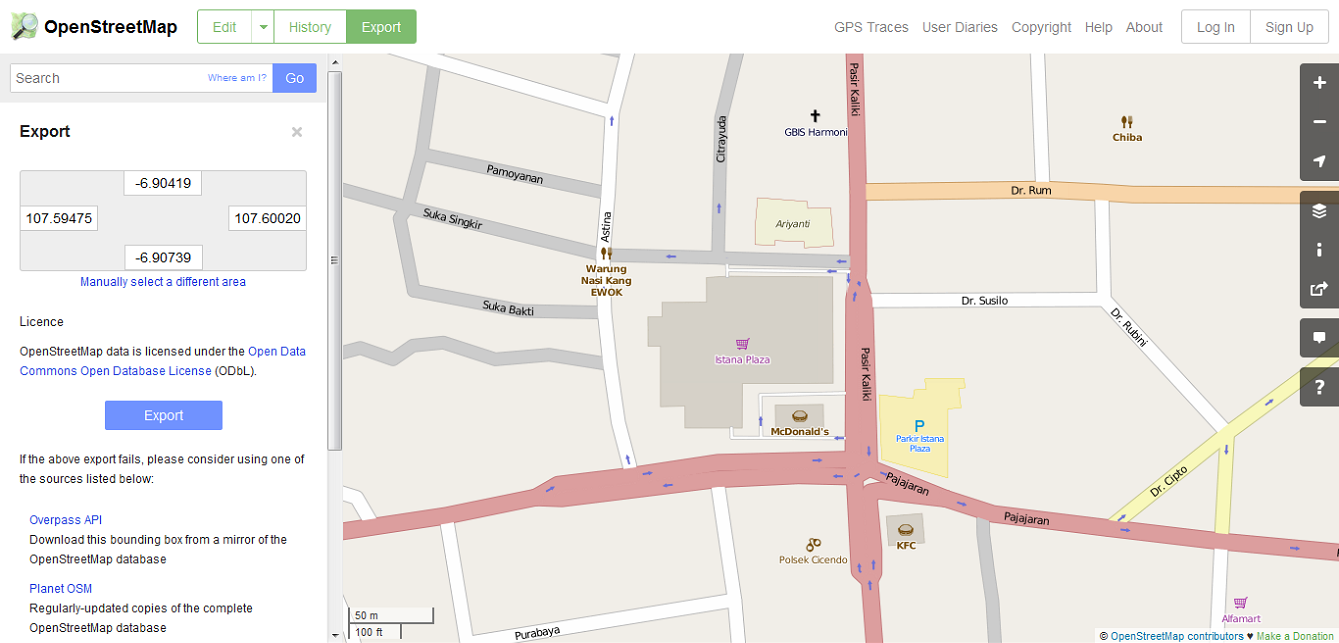
\includegraphics[scale=0.4]{Gambar/export_osm}
\caption[Ekspor data pada situs OpenStreetMap]{Ekspor data pada situs
OpenStreetMap}
\label{fig:export_osm}
\end{figure}

Berikut ini adalah beberapa data yang dapat diambil menggunakan fitur export
\cite{wiki:001}:
\begin{enumerate}
\item OpenStreetMap XML Data

OSM XML data dapat diperoleh dengan cara menggunakan tombol Export di bagian atas untuk 
membuka sidebar. Tombol Export mengarahkan langsung browser kepada OpenStreetMap API yang 
menyediakan data mentah OSM dalam bentuk XML.

\item Mapnik \textit{Image} 

Memungkinkan ekspor data OSM dalam bentuk PNG, JPEG, SVG, PDF dan peta PostScript.

\item \textit{Embeddable} HTML

Fitur ini memungkinkan pengguna untuk mendapatkan kode HTML yang dapat disalin dan digunakan pada halaman web lain. Kode HTML tersebut akan menyisipkan peta dalam sebuah iframe lengkap dengan javascript.
\end{enumerate}

\section{XML}
XML adalah singkatan dari eXtensible Markup Language, XML adalah bahasa markup 
yang dikembangkan oleh W3C (World Wide Web Consortium)
\cite{Benoit:2000}. Berikut ini adalah contoh dokumen XML:
\lstset{basicstyle=\normalsize}
\begin{lstlisting}
<?xml version="1.0" encoding="utf-8"?>
  <catalog>
   <book id="bk101">
      <author>Gambardella, Matthew</author>
      <title>XML Developer's Guide</title>
      <genre>Computer</genre>
      <price>44.95</price>
      <publish_date>2000-10-01</publish_date>
      <description>An in-depth look at creating applications 
      with XML.</description>
   </book>
   <book id="bk102">
      <author>Ralls, Kim</author>
      <title>Midnight Rain</title>
      <genre>Fantasy</genre>
      <price>5.95</price>
      <publish_date>2000-12-16</publish_date>
      <description>A former architect battles corporate zombies, 
      an evil sorceress, and her own childhood to become queen 
      of the world.</description>
   </book>
  <catalog>
\end{lstlisting}
Contoh di atas memberikan informasi mengenai katalog buku yang disimpan pada
dokumen XML. Pada awal dokumen tertera versi XML dan \textit{encoding} yang
digunakan. Setelah itu, terdapat tag catalog yang memiliki \textit{child} yaitu
tag buku beserta informasinya. Terdapat informasi id buku yang tertera pada atribut tag buku,
seperti <book id="bk101">. Dan juga informasi lain seperti judul buku, penulis,
genre, harga, tanggal terbit, dan deskripsi.

XML dikembangkan terutama 
untuk mengatasi keterbatasan pada HTML (Hypertext Markup Language). HTML adalah 
salah satu bahasa markup yang paling populer dan terus dikembangkan, banyak tag baru 
yang diperkenalkan. Pada versi pertama, HTML memiliki satu lusin tag dan pada
HTML pada versi 4.0 sudah hampir mencapai seratus tag. Namun, pada aplikasi
seperti \textit{electronic commerce} dibutuhkan tag lebih untuk produk, harga, nama,
alamat, dan banyak lagi atau situs \textit{streaming} memerlukan tag lebih untuk
mengontrol gambar dan suara.
\lstset{language=XML}

HTML telah berkembang menjadi bahasa yang cukup kompleks, W3C memperkirakan
penggunaan komputer akan terus berkurang dan penggunaan gadget seperti smartphone 
akan bertambah. Mesin tersebut tidak sekuat PC dan tidak bisa memproses bahasa yang 
kompleks seperti HTML . Meskipun HTML adalah bahasa yang populer dan cukup sukses, HTML 
memiliki beberapa kelemahan utama dan XML dikembangkan untuk mengatasi kelemahan tersebut. 
XML adalah bahasa yang digunakan untuk menggambarkan dan memanipulasi dokumen
terstruktur. Perubahan utama pada XML adalah tidak adanya tag yang ditetapkan pada XML. 
Karena tidak ada tag yang ditetapkan, penulis dapat membuat tag yang dibutuhkan. 
Beberapa ketentuan pada XML dapat dilihat pada uraian berikut:
\begin{enumerate}
\item Tag pada XML \\
Setiap elemen pada XML terdiri dari nama dan nilai, selain itu harus memiliki
tag pembuka dan tag penutup. Contoh: 
\begin{verbatim}
<tel> 513-555-7098 </ tel>
\end{verbatim}
Elemen untuk menyimpan nomor telepon memiliki nama tag tel, ditulis dengan <tel>
dan ditutup dengan </tel>.

\item Nama pada XML \\
Pemberian nama pada XML harus dimulai dengan huruf atau underscore (\_) dan
sisanya diikuti huruf, angka, atau titik. Spasi tidak diperbolehkan pada
pemberian nama.

\item Atribut \\
Atribut memungkinkan untuk menyisipkan informasi tambahan, atribut juga memiliki
nama dan nilai. Contoh:
\begin{verbatim}
<tel preferred="true">513-555-8889</tel>
<tel>513-555-7098</tel>
\end{verbatim}
Elemen tel dapat memiliki atribut \textit{preferred}, memberikan informasi nomor
telepon yang lebih sering digunakan.

\item Elemen Kosong \\
Elemen yang tidak memiliki nilai atau isi disebut sebagai elemen kosong. Elemen
kosong biasanya memiliki atribut. Contoh:
\begin{verbatim}
<email href="mailto:jdoe@emailaholic.com"></email>
\end{verbatim}
Elemen email tidak memiliki nilai atau isi.

\item \textit{Nesting of Elements} \\
Sebuah elemen dapat memiliki elemen lain di dalamnya. Elemen yang berada di
dalam elemen lain disebut \textit{child}, sedangkan elemen yang memiliki elemen
lain disebut \textit{parent}. Contoh
\begin{verbatim}
<name>
  <fname>Jack</fname>
  <lname>Smith</lname>
</name>
\end{verbatim}
Pada contoh berikut elemen name memiliki dua
\textit{child} yaitu fname dan lname dan elemen name merupakan \textit{parent}
dari kedua elemen tersebut.

\item \textit{Root} \\
\textit{Root} merupakan elemen pada level tertinggi dan pada dokumen XML harus
ada satu elemen pada level tertinggi. Dengan kata lain, elemen lain harus menjadi
\textit{child} dari \textit{root}.

\item Deklarasi XML \\
Deklarasi XML dituliskan pada baris pertama dokumen. Pada deklarasi tersebut
juga dituliskan versi XML yang digunakan. Contoh:
\begin{verbatim}
<?xml version="1.0"?>
\end{verbatim}
\end{enumerate}

\subsection{OSMXML}
OpenStreetMap XML atau biasa disingkat dengan OSMXML merupakan dokumen XML yang
berisi data-data peta OSM. Pada dasarnya, OSMXML berisi data primitif
(node, way, dan relation) yang merupakan arsitektur dari model OSM
\cite{wiki:001}.
Berikut ini adalah contoh dokumen OSMXML:
\lstset{
  language=XML,
  morekeywords={osm,bounds,node,way,relation,tag,nd,member}
}
\begin{lstlisting}
<?xml version="1.0" encoding="UTF-8"?>
<osm version="0.6" generator="CGImap 0.0.2">
 <bounds minlat="54.0889580" minlon="12.2487570" maxlat="54.0913900" maxlon="12.2524800"/>
 <node id="298884269" lat="54.0901746" lon="12.2482632" user="SvenHRO" uid="46882" visible="true" version="1" changeset="676636" timestamp="2008-09-21T21:37:45Z"/>
 <node id="261728686" lat="54.0906309" lon="12.2441924" user="PikoWinter" uid="36744" visible="true" version="1" changeset="323878" timestamp="2008-05-03T13:39:23Z"/>
 <node id="1831881213" version="1" changeset="12370172" lat="54.0900666" lon="12.2539381" user="lafkor" uid="75625" visible="true" timestamp="2012-07-20T09:43:19Z">
  <tag k="name" v="Neu Broderstorf"/>
  <tag k="traffic_sign" v="city_limit"/>
 </node>
 ...
 <node id="298884272" lat="54.0901447" lon="12.2516513" user="SvenHRO" uid="46882" visible="true" version="1" changeset="676636" timestamp="2008-09-21T21:37:45Z"/>
 <way id="26659127" user="Masch" uid="55988" visible="true" version="5" changeset="4142606" timestamp="2010-03-16T11:47:08Z">
  <nd ref="292403538"/>
  <nd ref="298884289"/>
  ...
  <nd ref="261728686"/>
  <tag k="highway" v="unclassified"/>
  <tag k="name" v="Pastower Straße"/>
 </way>
 <relation id="56688" user="kmvar" uid="56190" visible="true" version="28" changeset="6947637" timestamp="2011-01-12T14:23:49Z">
  <member type="node" ref="294942404" role=""/>
  ...
  <member type="node" ref="364933006" role=""/>
  <member type="way" ref="4579143" role=""/>
  ...
  <member type="node" ref="249673494" role=""/>
  <tag k="name" v="Küstenbus Linie 123"/>
  <tag k="network" v="VVW"/>
  <tag k="operator" v="Regionalverkehr Küste"/>
  <tag k="ref" v="123"/>
  <tag k="route" v="bus"/>
  <tag k="type" v="route"/>
 </relation>
 ...
</osm>
\end{lstlisting}
Struktur OSMXML:
\begin{itemize}
\item Dokumen OSMXML diawali dengan tag xml yang menjelaskan versi xml dan
encoding yang digunakan, pada contoh di atas digunakan xml versi 1.0 dan
encoding UTF-8.

\item Elemen osm memberikan informasi mengenai versi API dan generator yang
digunakan. Generator adalah alat untuk membuat dokumen XML pada saat fitur
export digunakan. 

\item Elemen bound memberikan informasi mengenai cakupan area pada dokumen XML
tersebut. Dilengkapi dengan atribut koordinat yaitu latitude dan longitude.
Data primitif pada OSM dibagi menjadi 3 bagian, yaitu node, way, dan relation.
\begin{enumerate}
\item Elemen Node merupakan informasi titik pada sebuah peta. Node memiliki
beberapa atribut yaitu:
\begin{itemize}
\item id \\
Merupakan id dari node tersebut.

\item user \\ 
Merupakan user yang melakukan editing pada node.

\item uid \\
Id dari user.

\item lat \\
berisi informasi koordinat pada garis lintang.

\item lon \\
berisi informasi koordinat pada garis bujur.

\item timestamp \\
Berisi informasi waktu saat node tersebut diperbaharui.
\end{itemize}
Node juga memiliki elemen tag sebagai \textit{child} yang memberikan informasi
tambahan pada node tersebut, contoh:
\begin{verbatim}
<tag k="name" v="Neu Broderstorf"/>
\end{verbatim}
nama dari node tersebut adalah Neu Broderstorf.

\item Elemen Way merupakan informasi garis yang dapat diartikan sebagai jalan
ataupun elemen lain seperti rel kereta pada peta OSM. Way menyimpan informasi
node-node yang dilalui oleh garis dan juga sama seperti node dilengkapi atribut seperti id, uid, user, changeset,
timestamp. Elemen way memiliki \textit{child} elemen nd, contoh:  
\begin{verbatim}
<nd ref="292403538"/>
\end{verbatim}
atribut ref pada elemen nd mengacu pada node yang memiliki id 292403538, dan
elemen tag yang memberikan informasi tambahan pada elemen way,

\item Elemen relation menyimpan informasi node-node dan way yang bersinggungan.
Elemen relation dapat menggambarkan suatu area seperti lapangan, taman bermain, atau
pada contoh di atas menggambarkan rute bus.
\end{enumerate}
\end{itemize}

\section{Javascript}
Javascript adalah bahasa pemrograman web yang mulai dikembangkan di perusahaan
yang bernama Netscape. Javascript memiliki lisensi dari Sun Microsystems yang sekarang sudah berganti nama 
menjadi Oracle. Saat ini, mayoritas situs web sudah menggunakan javascript.
Berikut ini adalah contoh penggunaan javascript pada dokumen HTML:
\lstset{
  language=HTML
}
\begin{lstlisting}
<!DOCTYPE html>
<html>
<head>
<script>
function myFunction() {
    document.getElementById("demo").innerHTML = "Paragraph changed.";
}
</script>
</head>
<body>
<h1>JavaScript in Head</h1>
<p id="demo">A Paragraph.</p>
<button type="button" onclick="myFunction()">Try it</button>
</body>
</html> 
\end{lstlisting}
Pada contoh di atas terdapat fungsi yang ditulis menggunakan javascript,
fungsi tersebut akan mengubah string ``A Paragraph'' pada tag <p> menjadi
``Paragraph changed'' jika \textit{button} atau tombol ``Try it'' di klik.

Seluruh browser yang terdapat pada komputer, konsol game, tablet, dan smartphone
sudah disertai dengan javascript interpreter. Interpreter adalah suatu program yang berfungsi 
untuk menerjemahkan kode program ke dalam bahasa mesin. Javascript adalah bagian yang 
cukup penting pada sebuah halaman web, jika HTML 
berfungsi untuk menentukan isi dari halaman dan CSS untuk menentukan tampilan pada halaman, javascript 
berfungsi untuk menentukan ``behavior'' dari halaman web tersebut
\cite{Flanagan:2011}.
Berikut ini adalah uraian dari struktur javascript dan beberapa contoh sintaks:
\begin{enumerate}
\item Struktur

\begin{itemize}
\item \textit{Character Set} \\
Javascript ditulis menggunakan karakter Unicode. Unicode adalah superset ASCII dan Latin-1 yang mendukung 
hampir seluruh bahasa di dunia.

\item \textit{Comments} \\
Javascript mendukung 2 jenis komentar yaitu komentar yang diletakkan setelah garis miring ganda // dan komentar yang 
diletakkan antara karakter /* dan */.
\begin{verbatim}
// This is a single-line comment.
/* This is also a comment */ // and here is another comment.
/*
* This is yet another comment.
* It has multiple lines.
*/
\end{verbatim}

\item Literal \\
Literal adalah notasi untuk merepresentasikan nilai 
dan nilai yang dituliskan akan muncul secara langsung dalam program. Literal
dapat berupa karakter, bilangan bulat, bilangan real, boolean. Berikut
ini adalah contoh literal:
\begin{verbatim}
12 // The number twelve
1.2 // The number one point two
"hello world" // A string of text
'Hi' // Another string
true // A Boolean value
false // The other Boolean value
/javascript/gi // A "regular expression" literal (for pattern matching)
null // Absence of an object 
\end{verbatim}

\item \textit{Identifier} \\
\textit{Identifier} pada javascript hanyalah nama yang digunakan untuk memberi
nama pada variabel atau fungsi. Digit tidak diperbolehkan sebagai karakter
pertama pada \textit{identifier}.

\item \textit{Reserved words} \\
\textit{Reserved words} adalah kata-kata yang tidak dapat digunakan sebagai
identifier, karena digunakan oleh javascript sebagai keyword. Beberapa contoh keyword seperti break, delete, if, 
null, true, false, try, dan lain-lain.

\item \textit{Optional Semicolons} \\
Seperti banyak bahasa pemrograman lain, javascript menggunakan titik koma (;) untuk memisahkan perintah 
yang ditulis. Hal ini penting untuk membuat kode program menjadi jelas mengenai awal dan akhir. Pada 
javascript, titik koma dapat dihilangkan jika perintah ditulis pada baris yang berbeda, berikut adalah 
contoh penggunaan titik koma pada javascript:
\begin{verbatim}
a = 3;
b = 4;
\end{verbatim}
titik koma pertama dapat dihilangkan, namun jika ditulis pada baris yang sama, titik koma tetap diperlukan
\begin{verbatim}
a = 3; b = 4;
\end{verbatim}
\end{itemize}

\item Sintaks
\begin{itemize}
\item Deklarasi Variabel \\
Pembuatan variabel pada javascript menggunakan keyword var. Contoh deklarasi atau pembuatan variabel pada javascript:
\begin{verbatim}
var i;
var i, sum;
var message = "hello";
var i = 0, j = 0, k = 0;
\end{verbatim}


\item Fungsi \\
Fungsi adalah blok kode program yang hanya didefinisikan sekali, tapi dapat
dipanggil atau dijalankan berulang kali. Pada javascript, fungsi dapat dibuat menggunakan keyword function. 
Sebuah fungsi harus memiliki nama, sepasang tanda kurung untuk parameter, dan sepasang kurung kurawal. 
Berikut ini adalah beberapa contoh fungsi:
\begin{verbatim}
// Print the name and value of each property of o. Return undefined.
function printprops(o) {
  for(var p in o)
    console.log(p + ": " + o[p] + "\n");
}
\end{verbatim}
\begin{verbatim}
// Compute the distance between Cartesian points (x1,y1) and (x2,y2).
function distance(x1, y1, x2, y2) {
  var dx = x2 - x1;
  var dy = y2 - y1;
  return Math.sqrt(dx*dx + dy*dy);
}
\end{verbatim}
\end{itemize}
\end{enumerate}

\subsection{XMLHttpRequest}
XMLHttpRequest adalah salah satu objek pada javascript yang dapat digunakan
untuk mendapatkan \textit{file} XML dari \textit{server} secara \textit{asynchronous}
atau \textit{synchronous} \cite{Edmond:2006}. \textit{Asynchronous} berarti
bahwa pertukaran data dilakukan tanpa harus memuat ulang seluruh halaman \textit{web}, sedangkan 
pertukaran data \textit{synchronous} harus memuat ulang seluruh halaman
\textit{web}. Berikut ini adalah contoh penggunaan XMLHttpRequest:
\begin{verbatim}
var objXMLHTTP = new XMLHttpRequest();

objXMLHTTP.open('GET', 'books.xml', false);
objXMLHTTP.send(null);

var objXML = objXMLHTTP.responseXML;
\end{verbatim}
Langkah pertama adalah dengan membuat objek XMLHttpRequest. Selanjutnya, dengan
memanggil fungsi open(``method'', ``url'', asynchronous). Parameter
\textit{method} menentukan metode yang digunakan, contoh ``GET'' untuk menerima
data dan ``POST'' untuk mengirim data, parameter url adalah alamat
\textit{file}, dan parameter boolean ``false'' menunjukkan bahwa permintaan tersebut
dilakukan secara \textit{synchronous}. Langkah terakhir adalah mendapatkan
respon dari \textit{server}

\subsection{XML DOM}
DOM adalah singkatan dari \textit{Document Object Model}, XML DOM adalah API
umum untuk menangani dokumen XML \cite{Edmond:2006}. API adalah singkatan dari
\textit{Application Programming Interface} merupakan fungsi atau perintah yang dapat digunakan untuk
menangani masalah pemrograman tertentu. XML DOM menyediakan fungsi standar
untuk mengakses, memodifikasi, dan menciptakan berbagai bagian dari sebuah dokumen XML.
Contoh:
\begin{verbatim}
var myNodeset = objXML.getElementsByTagName('plant');
\end{verbatim}
Pemanggilan fungsi getElementsByTagName('plant') akan mengembalikan satu set
node yang memiliki nama tag 'plant'. Contoh lain, pemanggilan fungsi
.getAttribute() akan mengembalikan nilai atribut.

\subsection{Google Maps Javascript API}
Google Maps Javascript API memungkinkan untuk sebuah halaman web menampilkan
peta dunia yang datanya didapat dari server google \cite{gmap:001}. Google
menyediakan fungsi atau perintah untuk menampilkan dan menyesuaikan peta sesuai dengan
kebutuhan. Berikut ini adalah contoh halaman web yang menampilkan peta di lokasi
Sydney, Australia:
\lstset{
  language=HTML
}
\begin{lstlisting}
<!DOCTYPE html>
<html>
  <head>
    <style type="text/css">
      html, body, #map-canvas { height: 100%; margin: 0; padding: 0;}
    </style>
    <script type="text/javascript"
      src="https://maps.googleapis.com/maps/api/js?key=API_KEY">
    </script>
    <script type="text/javascript">
      function initialize() {
        var mapOptions = {
          center: { lat: -34.397, lng: 150.644},
          zoom: 8
        };
        var map = new google.maps.Map(document.getElementById('map-canvas'),
            mapOptions);
      }
      google.maps.event.addDomListener(window, 'load', initialize);
    </script>
  </head>
  <body>
<div id="map-canvas"></div>
  </body>
</html>
\end{lstlisting}
\begin{itemize}
\item Declaring \\
Google menyarankan untuk membuat deklarasi tipe dokumen pada awal dokumen yaitu
dengan menulis <!DOCTYPE html>. Setelah itu diperlukan CSS yang bekerja untuk
mengatur tampilan peta pada halaman web.
\begin{verbatim}
<style type="text/css">
  html { height: 100% }
  body { height: 100%; margin: 0; padding: 0 }
  #map-canvas { height: 100% }
</style>
\end{verbatim}
Kode CSS pada contoh menunjukkan tag yang memiliki id map-canvas akan memiliki
tinggi 100\% pada saat ditampilkan dan juga menunjukkan persentase yang sama
pada <html> dan <body>.

\item Loading Google Maps API\\
Untuk dapat menampilkan peta diperlukan juga melakukan \textit{load} javascript.
URL yang terdapat pada tag script adalah lokasi file javascript yang akan memuat
seluruh simbol dan definisi yang dibutuhkan untuk menggunakan Google Maps API
ini. Paramater key berisi API key yang dimiliki oleh pengguna.
\begin{verbatim}
<html>
  <head>
    <script type="text/javascript"
      src="https://maps.googleapis.com/maps/api/js?key=API_KEY">
    </script>
\end{verbatim}

\item Initialize \\
Setelah melakukan load javascript, diperlukan pemanggilan fungsi initialize. Di
dalam fungsi tersebut dapat ditambahkan beberapa variabel yang dibutuhkan.
\begin{verbatim}
function initialize() {}
\end{verbatim}
Untuk inisialisasi peta, diperlukan variabel map options
\begin{verbatim}
var mapOptions = {};
\end{verbatim}
Selanjutnya diperlukan koordinat pusat peta yang akan ditampilkan, sedangkan
zoom menunjukkan level zoom yang ingin ditampilkan
\begin{verbatim}
center: new google.maps.LatLng(-34.397, 150.644),
zoom: 8
\end{verbatim}

\item Map Object \\
Obyek peta perlu dibuat dengan cara melakukan inisialisasi kelas
google.maps.Map. Pada contoh, peta diletakkan pada <div> yang memiliki id
map-canvas.
\begin{verbatim}
var map = new google.maps.Map(document.getElementById("map-canvas"),
    mapOptions);
\end{verbatim}

\item Loading the Map \\
Google Maps API menyediakan fungsi untuk memuat peta 
\begin{verbatim}
google.maps.event.addDomListener(window, 'load', initialize);
\end{verbatim}
\end{itemize}

\setcounter{secnumdepth}{3}
\setcounter{tocdepth}{3}
\subsubsection{Menggambar pada Peta}
Peta pada Google Maps API dapat ditambahkan objek seperti titik, garis, area,
atau objek lainnya. Objek tersebut dinamakan \textit{overlay}. Terdapat beberapa
jenis \textit{overlay} yang dapat ditambahkan pada peta yaitu sebagai berikut: 
\begin{enumerate}
\item \textit{Marker} \\
Lokasi tunggal pada peta ditunjukkan oleh \textit{Marker}.
\begin{itemize}
  \item Menambahkan \textit{Marker} \\
  Untuk menampilkan \textit{marker} pada peta harus membuat objek
  google.maps.Marker. Berikut ini adalah atribut penting pada saat
  membuat objek \textit{marker}:
  \begin{enumerate}
    \item \textit{position} \\
    atribut \textit{position} diperlukan untuk mengatur letak \textit{marker}
    pada peta.
    
    \item \textit{map} \\
    atribut \textit{map} bersifat opsional, untuk menentukan marker
    tersebut akan diletakkan pada peta. Jika atribut \textit{map} tidak diatur,
    maka \textit{marker} akan tetap dibuat tetapi tidak akan ditampilkan pada
    peta.
  \end{enumerate}
  Berikut ini adalah contoh kode program untuk menambahkan \textit{marker} pada
  peta:
  \begin{verbatim}
var myLatlng = new google.maps.LatLng(-25.363882,131.044922);
	var mapOptions = {
	  zoom: 4,
	  center: myLatlng
	}
	var map = new google.maps.Map(document.getElementById
	("map-canvas"), mapOptions);
	
	// To add the marker to the map, use the 'map' property
	var marker = new google.maps.Marker({
	    position: myLatlng,
	    map: map,
	    title:"Hello World!"
	});
  \end{verbatim}
  Pada contoh, objek google.maps.Marker yang dibuat disimpan pada variabel
  marker, terdapat atribut \textit{position} menggunakan variabel myLatlng
  yang berisi koordinat (-25.363882,131.044922), atribut map menunjukkan bahwa
  \textit{marker} akan ditampilkan pada objek map yang tersimpan pada variabel
  map, dan atribut yang menunjukkan judul \textit{marker}. 
  
  \item Menghapus \textit{Marker} pada peta\\
  Untuk menghapus \textit{marker} pada peta, hanya diperlukan pemanggilan
  fungsi setMap() dan mengisi parameter fungsi tersebut dengan \textit{null}.
  Contoh:
  \begin{verbatim}
marker.setMap(null);
  \end{verbatim}
  Pada contoh di atas hanya menghilangkan \textit{marker} dari peta dan tidak
  menghapus objek \textit{marker}.
  
  \item Animasi \textit{Marker} \\
  Menambahkan animasi pada \textit{marker}, hanya memerlukan pengaturan atribut
  pada konstruktor google.maps.Marker. Contoh:
  \begin{verbatim}
  var marker = new google.maps.Marker({
	    position: myLatlng,
	    map: map,
	    animation: google.maps.Animation.BOUNCE,
	    title:"Hello World!"
	});
  \end{verbatim}
  Pada contoh, menambahkan animasi \textit{bounce} pada marker sehingga
  \textit{marker} bergerak melompat-lompat pada peta. 
  
  \item Mengubah Ikon \\
  Gambar \textit{marker} pada peta dapat diubah sesuai keinginan, hanya
  memerlukan pengaturan atribut pada konstruktor google.maps.Marker. Contoh:
  \begin{verbatim}
  var image = 'images/beachflag.png';
  var myLatLng = new google.maps.LatLng(-33.890542, 151.274856);
  var beachMarker = new google.maps.Marker({
      position: myLatLng,
      map: map,
      icon: image
  });
  \end{verbatim}
  Pada contoh, ikon \textit{marker} akan ditampilkan menggunakan \textit{file}
  gambar beachflag.png
  
  \item \textit{Draggable} \\
  Draggable memungkinkan pengguna untuk menyeret marker ke lokasi yang berbeda,
  hanya memerlukan pengaturan atribut pada konstruktor google.maps.Marker. Contoh:
  \begin{verbatim}
  var marker = new google.maps.Marker({
	    position: myLatlng,
	    map: map,
	    draggable: true,
	    title:"Hello World!"
	});
  \end{verbatim}
\end{itemize}
\item \textit{Polyline} \\
Objek \textit{polyline} adalah serangkaian garis pada peta, \textit{polyline}
berguna untuk menunjukkan dari satu titik ke titik lain. \textit{Polyline}
memiliki atribut yang dapat diubah sesuai kebutuhan seperti warna,
\textit{opacity}, dan \textit{weight}. Berikut ini penjelasan dari
beberapa atribut tersebut:
\begin{itemize}
  \item \textit{strokeColor} \\
  Atribut \textit{strokeColor} menentukan warna dalam format
  heksadesimal, contoh \\ "\#FFFFFF''.
  
  \item \textit{strokeOpacity} \\
  Atribut \textit{strokeOpacity} menentukan \textit{opacity} dalam nilai antara
  0.0 dan 1.0.
  
  \item \textit{strokeWeight} \\
  Atribut \textit{strokeWeight} menentukan lebar garis dalam piksel.
\end{itemize}
Berikut ini adalah contoh potongan kode program untuk menampilkan
\textit{polyline} pada peta:
\begin{verbatim}
var flightPlanCoordinates = [
    new google.maps.LatLng(37.772323, -122.214897),
    new google.maps.LatLng(21.291982, -157.821856),
    new google.maps.LatLng(-18.142599, 178.431),
    new google.maps.LatLng(-27.46758, 153.027892)
  ];
  var flightPath = new google.maps.Polyline({
    path: flightPlanCoordinates,
    strokeColor: '#FF0000',
    strokeOpacity: 1.0,
    strokeWeight: 2
  });

  flightPath.setMap(map);
\end{verbatim}
Pada contoh, akan menampilkan polyline pada peta yang akan menghubungkan setiap 
koordinat yang terdapat pada variabel flightPlanCoordinates. \textit{Polyline}
yang ditampilkan pada peta dapat dilihat pada Gambar \ref{fig:polyline}.
\begin{figure}[h]
\centering
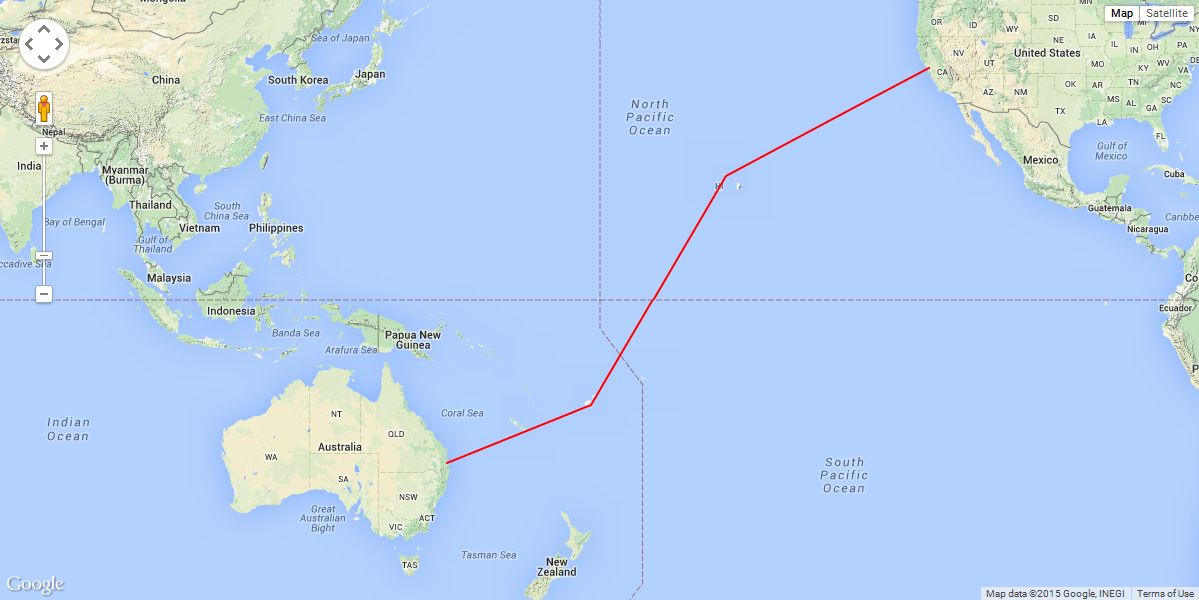
\includegraphics[scale=0.4]{Gambar/polyline}
\caption[Polyline pada Peta]{Polyline pada Peta}
\label{fig:polyline}
\end{figure}
\end{enumerate}

\section{Graf}
Graf adalah himpunan obyek yang terrdiri dari simpul (node) dan sisi (edge), graf 
digambarkan sebagai node yang dihubungkan oleh edge. Konsep graf telah digunakan pada 
banyak aplikasi komputer dan menggunakan beberapa jenis graf seperti graf sederhana, graf 
tidak berarah, graf berarah, graf tak terbatas, dan lain-lain. Contoh graf dapat
dilihat pada Gambar \ref{fig:graph}. Graf mengikuti aturan berikut
\footnotemark[2]:
\begin{enumerate}
\item Graf terdiri dari dua bagian yang disebut simpul dan sisi.
\item Node digambarkan berdasarkan tipenya dan nilainya mungkin terbatas atau
tidak terbatas. 
\item Setiap sisi menghubungkan dua buah simpul.
\item Node digambarkan sebagai kotak atau lingkaran dan edge digambarkan sebagai
garis atau busur.
\end{enumerate}
\begin{figure}[h]
\centering
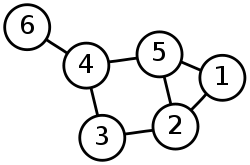
\includegraphics[scale=0.8]{Gambar/graph}
\caption[Contoh Graf]{Contoh Graf}
\label{fig:graph}
\end{figure}
Berdasarkan contoh pada Gambar \ref{fig:graph}  didapatkan informasi tipe dari
simpul adalah bilangan bulat \\
Himpunan simpul = {1,2,3,4,5,6} \\ 
Himpunan edge = {(6,4),(4,5),(4,3),(3,2),(5,2),(2,1),(5,1)}

\subsection{Graf Berarah}
Graf berarah memiliki arah pada setiap edgenya. Pada graf berarah, edge biasanya
digambarkan dengan panah sesuai arahnya. Contoh graf berarah dapat dilihat pada
Gambar \ref{fig:direc_graph}.
\begin{figure}[h]
\centering
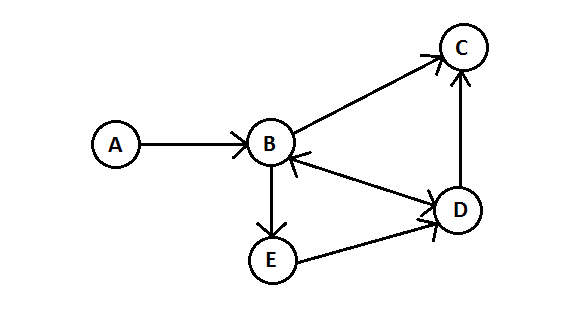
\includegraphics[scale=1]{Gambar/direc_graph}
\caption[Contoh Graf Berarah]{Contoh Graf Berarah}
\label{fig:direc_graph}
\end{figure}

Berdasarkan contoh pada Gambar \ref{fig:direc_graph}  didapatkan informasi tipe
dari simpul adalah huruf kapital \\
Himpunan simpul = {A, B, C, D, E} \\ 
Himpunan edge = {(A, B), (B, C), (D, C), (B, D), (D, B), (E, D), (B, E)}
\footnotetext[2]{http://web.cecs.pdx.edu/~sheard/course/Cs163/Doc/Graphs.html}

\section{Algoritma Dijkstra}
Algoritma dijkstra adalah algoritma yang dapat mencari jalur terpendek pada graf
berarah dengan persamaan G=(V,E) untuk kasus pada setiap sisinya bernilai tidak
negatif \cite{Cormen:2001}. Algoritma ini menggunakan prinsip greedy. Prinsip
greedy pada algoritma dijkstra menyatakan bahwa pada setiap langkahnya memilih sisi yang berbobot minimum dan
memasukannya dalam himpunan solusi. Berikut ini adalah langkah-langkah dari
algoritma dijkstra:
\begin{enumerate}
  \item Inisialisasi setiap node dengan nilai jarak sementara dan berikan nilai nol pada
node awal.

  \item Tandai node awal tersebut sebagai \textit{current} node dan tandai juga seluruh
node lainnya sebagai node yang belum dikunjungi (\textit{unvisited} set).
 
  \item Hitung jarak seluruh node yang bertetangga dengan \textit{current} node dengan
cara membandingkan jarak yang dimiliki \textit{current} node dan jarak tetangganya satu persatu, jika jarak yang dimiliki \textit{current} 
node lebih besar maka ganti nilai tersebut.

  \item Setelah selesai menghitung jarak seluruh tetangganya, hapus \textit{current} node
dari \textit{unvisited} set dan tandai bahwa node tersebut sudah dikunjungi.

  \item Selanjutnya, pilih node yang belum dikunjungi dengan nilai jarak
terkecil dan tandai node tersebut sebagai \textit{current} node dan ulangi langkah 3.
\end{enumerate}
